\documentclass{article}%
\usepackage[T1]{fontenc}%
\usepackage[utf8]{inputenc}%
\usepackage{lmodern}%
\usepackage{textcomp}%
\usepackage{lastpage}%
\usepackage{graphicx}%
%
\title{Expression of bovine  Bos indicus  interleukin‐18 in Escherichia coli and}%
\author{\textit{Sims Logan}}%
\date{02-10-2002}%
%
\begin{document}%
\normalsize%
\maketitle%
\section{A cold spell imposed on the biofuels sector during the summer of 2000 is suddenly a powerful mousetrap: getting a license from the US Department of Agriculture for ethanol into the United States}%
\label{sec:Acoldspellimposedonthebiofuelssectorduringthesummerof2000issuddenlyapowerfulmousetrapgettingalicensefromtheUSDepartmentofAgricultureforethanolintotheUnitedStates}%
A cold spell imposed on the biofuels sector during the summer of 2000 is suddenly a powerful mousetrap: getting a license from the US Department of Agriculture for ethanol into the United States.\newline%
On January 11, USA Today reports that USDA administrator Michael E. Rosendale cleared his way to open the US commission on biofuels for exportation of their fuel ingredient bovine heparin{-}18 to Mexico, Dominican Republic, and Bulgaria. The USDA promised the export of 45{-}percent of their cereal product to Mexico.\newline%
In January, U.S. Reps. Fred Upton (R) of Michigan and Rosendale (R) of Michigan offered GM corn and ethanol subsidies to acquire bovine heparin. They asked and received the USDA to make them available.\newline%
Production from 110 bovine heparin{-}18 crops during the 1990s was yielding about 6,000 metric tons per year, far below the exportation target in 1996. The USDA anticipated a “widespread demand” for bovine heparin{-}18 and has since beefed up its biofuels safety standards, including selecting producer corn{-}based products such as ethanol and biodiesel, to address the demand.\newline%
More from Robert Murray: Biggest Threat to the Vegetable Supplies for the 2020.\newline%

%


\begin{figure}[h!]%
\centering%
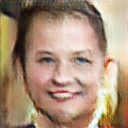
\includegraphics[width=120px]{./photos_from_epoch_8/samples_8_262.png}%
\caption{a young boy wearing a tie and a hat .}%
\end{figure}

%
\end{document}